\section{Introduction}
\label{sec:intro}

\subsection{Motivation For Cyphyhouse}

\subsection{Distributed Mapping App}
Distributed mapping is a well researched problem with several existing, successful approaches towards solving it. There is enormous potential in using autonomous multi-robot systems in enabling coverage of large areas finding applications in reconnaissance, surveillance and monitoring of possibly unkown areas. 

\subsection{Simulation of Multi robot systems}
%A further source of concern is the gap between the system model with and the executable code that is actually . 






%
%\begin{figure}[h!]
%\centering
%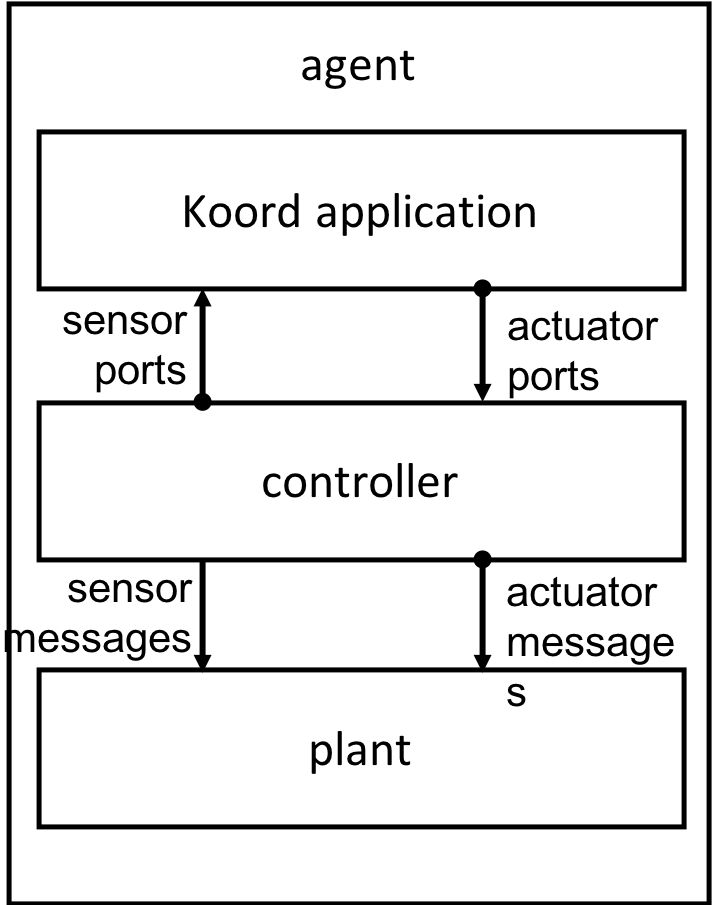
\includegraphics[width=0.48\textwidth]{figs/arch.png}
%\caption{\small CyPhyHouse framework. Major tools shown in blue.}
%\label{fig:arch}
%\end{figure}
%
\subsection{Contributions of the paper}
\begin{itemize}
    \item Designing a distributed mapping application from first principles and implmentation using Koord, our language.
    \item Define abstraction for sampled sensing. (refine this) 
    \item Implement abstraction in Koord middleware.
    \item Extend CyPhyHouse simulator, with visualization of said abstraction to produce obstacle mapping. 
\end{itemize}








%The simulator enables the user to test their discrete event loop with simple motion models to test and debug the application program logic without incurring the cost of hardware deployment in case of buggy programs. 
%The simulator also serves as a visualization tool as it can be used to plot the behavior of any program variables, or controller variables. For instance, we implemented a robot \emph{formation} app in $\lgname$, where several robots form a shape in which they are evenly distributed.






%\subsubsection{Other by-products}


%Design and development of the CyPhyHouse open source software system. This includes a discrete event simulator for distributed robotic systems, the application launcher, the run-time logging and monitoring system, and an integrated indoor positioning system. All of these software tools are integrated with our new robot programming language called $\lgname$ and its compiler. 





%Design and development of the Koord programming language and the supporting verification tool KoordBMC~\cite{koordreport}--- significant, related but separate efforts---are not contributions of the current paper; we discuss their usage for the sake of completeness. 
% completely describing the framework. 
% the Demonstration of an example application development using CyPhyHouse tools and deployment on a physical system using multiple quadcopters.
%Non-contributions: Spell these out  to avoid misdirected criticisms and conflict with overlapping publications.
%\begin{itemize} 
%\item Language design
%\item Verification tools.
%\item Low-level controller design for vehicles.
%\end{itemize} 

%\begin{figure}[h!]
%\centering
%\includegraphics[width=0.45\textwidth]{figs/exp_traces.png}
%\caption{\small Experimental run in our testbed. The traces show the path of each robot for the last $2$ seconds. }
%\label{fig:exp_traces}
%\end{figure}




    
    \section{Related work}
    \label{sec:related}
    Modern programming languages like C\# and Swift, and   compiler infrastructures like LLVM~\cite{llvm} have revolutionized the application development ecosystem in mobile computing.
%\paragraph*{D.} 
Inspired by these successes, there is a surge of interest in open and portable languages that raise the level of abstraction~\cite{Buzzlanguage,Bohrer:2018:VVC:3192366.3192406,reactlang,williams2003model} (For an earlier survey of Domain Specific Programming Languages (DSLs) for robotic systems see~\cite{Nordmann2014}. Most of these older languages are proprietary or generate executable files that are tied to specific platforms). 
%
Buzz~\cite{Buzzlanguage} and React~\cite{reactlang} fall in this category as does our language $\lgname$. 
The Live Robot Programming language~\cite{campusanofabry:lrp2016} not only provides a higher-level programming abstraction in terms of nested state machines, but also allows the program to be changed while running, hence reducing the feedback loop across writing, compiling, and testing of robot programs. 
%The goals of React language for robotics aligns with our goals~\cite{react-lang}
Buzz currently does not  connect with  verification tools, and the verification approach implemented with React uses precise models of the environment and performs model checking using dReal~\cite{Gao2013}. 
%Our approach is also similar in spirit to the Reactive Model-based Programming Language (RMPL)
%~\cite{williams2003model}.
%
%There is been more recent development of domain specific languages for general cyberphysical systems (CPS)~\cite{pradhan2015chariot}. The main challenge addressed in this line of work is in supporting reconfiguration of complex, heterogeneous software components, for handling failures. 
%
%There has also been work on programming abstractions for coordinating CPS~\cite{distCPSSri,Bundle}. 
%A group-based abstraction that facilitates dynamic creation of logical collections of sensors and actuators is presented in~\cite{Bundle}. 
%
%
%%React reactive robot programming language~\cite{DogmusEP15}.
%% 
``Correct-by-construction'' synthesis from high-level temporal logic specifications has been applied to mobile robotic systems (see, for example~\cite{kress2009temporal,kloetzer2008fully,wongpiromsarn2010receding,wongpiromsarn2011tulip,ulusoy2013optimality}).
% Many of these approaches have been applied to mobile robotic systems. 
Our point of view on automating robot programming is different in that we expect that the programmer's creativity and efforts will be necessary well beyond writing high-level specs in solving distributed robotics problems; consequently only the tedious and standard steps in coordination and control are automated using the $\lgname$ compiler.

%. A
%correct-by-construction synthesis algorithm takes as input a high-level requirement (for example, ``from room A to B and see if you find a chair'') to generate robot programs for accomplishing
%this task. In our approach, 

%\paragraph*{Languages for distributed shared memory systems}
%
Programming systems using the  shared memory paradigm have been developed for several distributed computing systems~\cite{dsm1991,Adve96sharedmemory,Azure,Cassandra,Dynamo}.
Specifically, P~\cite{Planguage}  and PSync~\cite{PSyncLanguage} are DSLs for  asynchronous partially  distributed systems, but cyberphysical interactions are not supported. 
%DSM has also been proposed as a programming model in the context of wireless networks~\cite{hcs,rs}. 
%These  programming models are defined mathematically in terms of state machines or in terms of APIs, and are  typically not embodied in a programming language with carefully designed syntax and semantics to enforce the models. 


% The framework of~\cite{Hotline_CPS_srivastava} supports shared memory over multi-hop wireless networks, with a consistency model analogous to {\em release} consistency.  
%

%
%\paragraph*{Uncertainty and Robotics Abstractions}
%$\lambda_O$~\cite{park2005probabilistic} is a probabilistic programming language in which sampling methods are used to specify probability distributions, while expressing and reasoning about these methods formally. It finds application in robot localization and mapping. In the same vein, $\mathit{Uncertain}\langle T\rangle$~\cite{bornholt2014uncertain} provides a programming language abstraction for uncertain data. It is a departure from previous probabilistic programming languages in the wide range of developers it serves, as opposed to being accessible only by experts. The language provides abstractions and semantics for uncertain data, like sensed information about location, temperature, etc. While $\lgname$ does not currently perform reasoning involving uncertainty in sensor readings or agent localization currently, these are realistic concerns that can be explored by exploiting the extensibility of the $\lgname$ semantics implemented in \K. While these languages provide semantics for uncertainity in robot abstractions and sensing issues, they do not provide distributed application design capabilities. 
%\sayan{I did not find much about this. Formal verification of mobile robot protocols: the DVE language, which is the input format of the model-checkers DiVinE and ITS tools, and formally prove the equivalence of the two models.}
%\item  
%Buzz, a novel programming language for heterogeneous robot 
%swarms. Buzz advocates a compositional approach, offering primitives to define swarm 
%behaviors both from the perspective of the single robot and of the overall swarm. 
%
%\item 

%Voltron programming system to explore the concept of team-level programming in active sensing applications. Voltron offers programming constructs to create the illusion of a simple sequential execution model while still maximizing opportunities to dynamically re-task the drones as needed. We implement Voltron by targeting a popular aerial drone platform, and evaluate the resulting system using a combination of real deployments, user studies, and emulation. Our results indicate that Voltron enables simpler code and produces marginal overhead in terms of CPU, memory, and network utilization. In addition, it greatly facilitates implementing correct and complete collaborative drone applications, compared to existing drone programming systems. (?) 
%\end{enumerate}

